\documentclass[../main.tex]{subfiles}

\begin{document}
\chapter{Extensive Form Games}
Let's introduce this new kind of "game" with an example:
\begin{example}
    Three politicians are supposed to decide whether to raise their salaries or not. The vote is public and in sequence. They would prefer to receive a salary increase, yet they would also like to vote against it so as not to lose public support.
\end{example}

Optimal result for each player: having salary increase while voting against it!

Main features of the game:
\begin{itemize}
    \item The moves take place in sequence: the politicians vote one after the other
    \item Every possible situation is known to the players: at any time they know the whole past history, as well as the possible developments
    \item The final outcome is determined by the majority of votes
\end{itemize}

This is an example of what is called a game with \textbf{perfect information}: each player has knowledge about all the events that have previously occurred.

\section{Games with perfect information}

How can we represent such a game? And how can we solve it?

Each player’s vote is represented at a branch: YES on the left and NO on the right. The game tree is the representation of the game in which each node is a possible situation and each edge is a possible move.

Utilities are based on individual votes and possible final outcomes:
1="YES and no raise"; 2="NO and no raise"; 3="YES and raise"; 4="NO and raise"
\begin{center}
    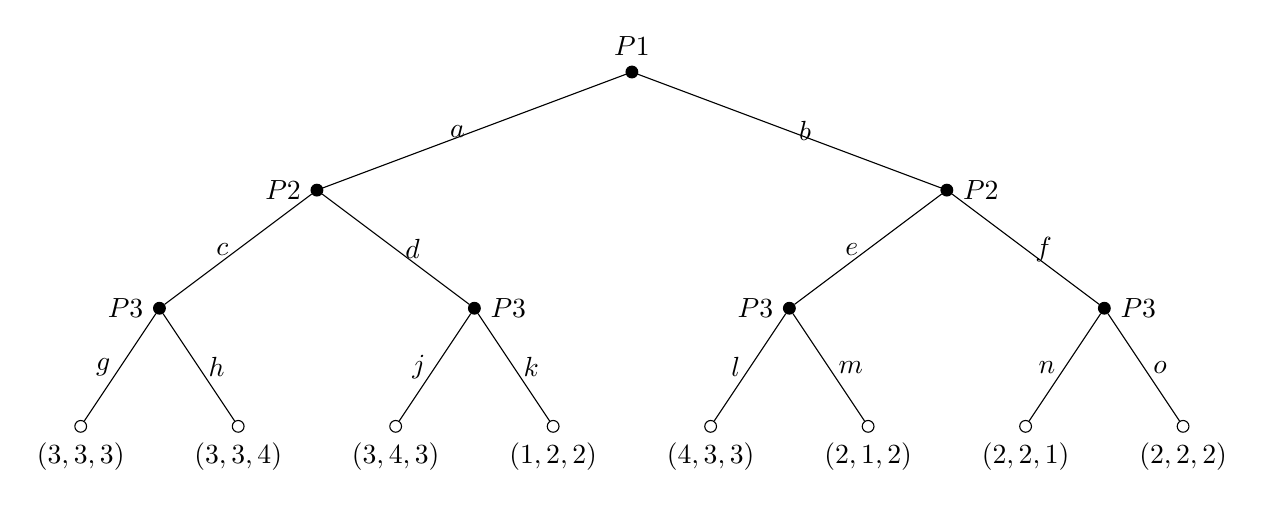
\begin{tikzpicture}
        \tikzstyle{solid node}=[circle,draw,inner sep=1.5,fill=black]
        \tikzstyle{hollow node}=[circle,draw,inner sep=1.5]
        \tikzstyle{level 1}=[level distance=15mm,sibling distance=8cm]
        \tikzstyle{level 2}=[level distance=15mm,sibling distance=4cm]
        \tikzstyle{level 3}=[level distance=15mm,sibling distance=2cm]

        \node(0)[solid node,label=above:{$P1$}]{}
        child{node[solid node,label=left:{$P2$}]{}
        child{node[solid node,label=left:{$P3$}]{}
        child{node[hollow node,label=below:{$(3,3,3)$}]{} edge from parent node[left]{$g$}}
        child{node[hollow node,label=below:{$(3,3,4)$}]{} edge from parent node[right]{$h$}}
        edge from parent node[left]{$c$}
        }
        child{node[solid node,label=right:{$P3$}]{}
        child{node[hollow node,label=below:{$(3,4,3)$}]{} edge from parent node[left]{$j$}}
        child{node[hollow node,label=below:{$(1,2,2)$}]{} edge from parent node[right]{$k$}}
        edge from parent node[right]{$d$}
        }
        edge from parent node[left]{$a$}
        }
        child{node[solid node,label=right:{$P2$}]{}
        child{node[solid node,label=left:{$P3$}]{}
        child{node[hollow node,label=below:{$(4,3,3)$}]{} edge from parent node[left]{$l$}}
        child{node[hollow node,label=below:{$(2,1,2)$}]{} edge from parent node[right]{$m$}}
        edge from parent node[left]{$e$}
        }
        child{node[solid node,label=right:{$P3$}]{}
        child{node[hollow node,label=below:{$(2,2,1)$}]{} edge from parent node[left]{$n$}}
        child{node[hollow node,label=below:{$(2,2,2)$}]{} edge from parent node[right]{$o$}}
        edge from parent node[right]{$f$}
        }
        edge from parent node[right]{$b$}
        };
    \end{tikzpicture}
\end{center}

We could also represent "chance" moves in the game tree
\begin{example}
    Two players 1 and 2 must decide in sequence whether to play or not.
    If both of them decide to play, then a coin is tossed (random component R): the first player wins with heads, whereas the second one with tails.
    \begin{center}
        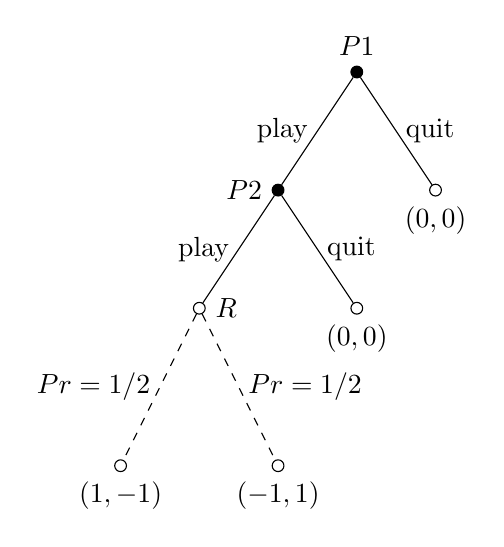
\begin{tikzpicture}
            \tikzstyle{solid node}=[circle,draw,inner sep=1.5,fill=black]
            \tikzstyle{hollow node}=[circle,draw,inner sep=1.5]
            \tikzstyle{level 1}=[level distance=15mm,sibling distance=20mm]
            \tikzstyle{level 2}=[level distance=15mm,sibling distance=20mm]
            \tikzstyle{level 3}=[level distance=20mm,sibling distance=20mm]

            \node(0)[solid node,label=above:{$P1$}]{}
            child{node[solid node,label=left:{$P2$}]{}
            child{node[hollow node,label=right:{$R$}]{}
            child{node[hollow node,label=below:{$(1,-1)$}]{}
            edge from parent[dashed] node[left]{$Pr = 1/2$}}
            child{node[hollow node,label=below:{$(-1,1)$}]{}
            edge from parent[dashed] node[right]{$Pr = 1/2$}}
            edge from parent node[left]{play}
            }
            child{node[hollow node,label=below:{$(0,0)$}]{}
            edge from parent node[right]{quit}}
            edge from parent node[left]{play}
            }
            child{node[hollow node,label=below:{$(0,0)$}]{}
            edge from parent node[right]{quit}
            };
        \end{tikzpicture}
    \end{center}
\end{example}

\begin{definition}[Finite Directed Graph]
    A finite directed graph is a pair $(V, E)$ where:
    \begin{itemize}
        \item $V$ is a finite set of vertices
        \item $E \subset V \times V$ is a set of ordered pairs of vertices called the set of directed edges
    \end{itemize}
\end{definition}
\begin{definition}
    A \textbf{path} from a vertex $v_1$ to a vertex $v_{k+1}$ is a finite sequence of vertices-edges: $v_1, e_1, v_2, e_2, \ldots, e_k, v_{k+1}$ such that $e_i \neq e_j$ for $i \neq j$ and $e_j = (v_j, v_{j+1})$. $k$ is called the \textbf{length} of the path
\end{definition}
\begin{definition}[Oriented Graph]
    An oriented graph is a finite directed graph having no bidirected edges, that is for all $j$, $k$ at most one between $(v_j , v_k)$ and $(v_k , v_j)$ may be arrows of the graph.
\end{definition}
\begin{definition}[Tree]
    A tree is a triple $(V, E, x_0)$ where $(V, E)$ is an oriented graph and $x_0 \in V$ is a vertex such that there is a unique path from $x_0$ to any other vertex
\end{definition}
\begin{definition}
    A \textbf{child} of a vertex $v$ is any vertex $x$ such that $(v, x) \in E$.

    A vertex is called a \textbf{leaf} if it has no children.

    We say that the vertex $x$ follows the vertex $v$ if there is a path from $v$ to $x$.
\end{definition}

\newpage % to avoid splitting the next definition

\begin{definition}[Extensive game with perfect information]
    An extensive game with perfect information consist of:
    \begin{itemize}
        \item A finite set $N=\{1,2,\ldots,n\}$ of players\footnote{The number $n$ denotes the cardinality of the set $N$}
        \item A game tree $(V, E, x_0)$
        \item A partition of the vertices that are not leaves into sets\footnote{For a partito into sets $P_i$ one has $V=\bigcup_{i=1}^{n+1} P_i$ and $P_i \cap P_j = \emptyset$ for $i \neq j$} ${P_1, P_2, \ldots, P_{n+1}}$
        \item A probability distribution for each vertex in $P_{n+1}$, defined on the edges from the vertex to its children
        \item A n-dimensional vector attached to each leaf (i.e. list of possible outcomes, i.e. the points associated to each player)
    \end{itemize}
\end{definition}

\begin{note}\
    \begin{itemize}
        \item The set $P_i$, for $i \leq n$, is the set of the nodes $v$ where Player $i$ must choose a child of $v$, representing a possible move from him at $v$
        \item $P_{n+1}$ is the set of the nodes where a chance move is present: that is $n+1$ is the number of players plus the random component. $P_{n+1}$ can be empty, meaning that the game does not admit any chance
        \item When $P_{n+1}$ is empty, the $n$ players have only preferences on the leaves: a utility function is not required
    \end{itemize}
\end{note}

\subsection{How to solve extensive form games}
In order to find the optimal outcome, we employ the \textbf{rationality axioms}:
\begin{itemize}
    \item What one player does when being in positions leading to leaves can be determined by decision theory (rationality assumption 5)
    \item This information is known to all other players (r.a. 4) that can use it
    \item Thus players moving to vertices going to leaves use decision theory (r.a. 5)
    \item This information is known to all other players (r.a. 4) that can be use it
    \item \ldots
    \item The player starting the game uses decision theory to make the first move
\end{itemize}

\begin{algorithm*}
    \caption*{Backward induction}
    \begin{itemize}
        \item Decision theory, i.e. rationality assumption 5, enables us to solve games of length 1
        \item Rationality assumption 4 allows us to solve a game of length $i + 1$ if the games of length at most $i$ are solved
    \end{itemize}
\end{algorithm*}

Thus, by repeated applications, we can solve games of any finite length.

This method takes the name of \textbf{backward induction}: it is the process of reasoning backwards in time (that is from the leaves of the tree up to the root), so as to determine a sequence of actions leading one to the optimal outcome.

\begin{definition}[Length of the Game]
    Define length of the game as the length of the longest path in the game
\end{definition}

\begin{theorem}[First Rationality Theorem]
    The rational outcomes of a finite, perfect information game are those given by the procedure of backward induction
\end{theorem}

The method of backwards induction can be applied since every vertex $v$ of the game is the root of a new game, made by all followers of $v$ in the initial game.

Such a game is called a \textbf{subgame} of the original one.

\begin{example}\
    \begin{center}
        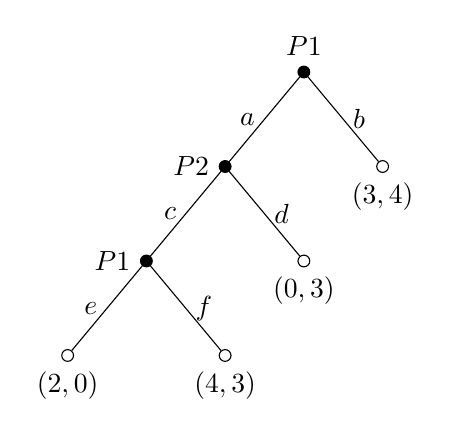
\begin{tikzpicture}
            \tikzstyle{solid node}=[circle,draw,inner sep=1.5,fill=black]
            \tikzstyle{hollow node}=[circle,draw,inner sep=1.5]
            \tikzstyle{level 1}=[level distance=12mm,sibling distance=20mm]
            \tikzstyle{level 2}=[level distance=12mm,sibling distance=20mm]
            \tikzstyle{level 3}=[level distance=12mm,sibling distance=20mm]

            \node(0)[solid node,label=above:{$P1$}]{}
            child{node[solid node,label=left:{$P2$}]{}
            child{node[solid node,label=left:{$P1$}]{}
            child{node[hollow node,label=below:{$(2,0)$}]{}
            edge from parent node[left]{$e$}}
            child{node[hollow node,label=below:{$(4,3)$}]{}
            edge from parent node[right]{$f$}}
            edge from parent node[left]{$c$}
            }
            child{node[hollow node,label=below:{$(0,3)$}]{}
            edge from parent node[right]{$d$}}
            edge from parent node[left]{$a$}
            }
            child{node[hollow node,label=below:{$(3,4)$}]{}
            edge from parent node[right]{$b$}
            };
        \end{tikzpicture}
    \end{center}
    The outcomes obtained by backward induction are: $(4, 3)$ and $(3, 4)$. In fact, Pl2 does not have any preference between $(4, 3)$ and $(0, 3)$!

    Therefore, in general, \textbf{uniqueness of solutions is not guaranteed}!
\end{example}

\subsection{Von Neumann's Chess Theorem}
\vspace{0.25cm}
\begin{theorem}
    In the game of chess one and only one of the following alternatives holds:
    \begin{enumerate}
        \item White has a winning strategy, no matter how Black plays
        \item Black has a winning strategy, no matter how White plays
        \item The white has a way to force at least a draw, no matter what the black does, and the same holds for the black
    \end{enumerate}
\end{theorem}

\begin{proof}
    Suppose the length of the game is $2k$ so each player has $k$ choices to make.
    Call $w_i$ the move of the White at her $i$-th stage and $b_i$ the one of the Black.
    The first alternative in the chess theorem can be written as:
    \begin{equation*}
        \exists w_1 : \forall b_1 \exists w_2 : \forall b_2 \ldots, \exists w_k : \forall b_k \implies \text{White wins}
    \end{equation*}
    Now suppose this is not true, then:
    \begin{equation*}
        \forall w_1\exists b_1 :  \forall w_2 \exists b_2 : \ldots, \forall w_K : \exists b_K \implies \text{White does not win}
    \end{equation*}
    This means that black has the possibility to get at least a draw.
\end{proof}

Summarizing:

if White does not have a strategy to win no matter what Black does, then Black has the possibility to get at least the draw.

Symmetrically, if Black does not have a strategy to win no matter what White does, then White has the possibility to get at least the draw.

Thus if the first and the second alternatives in the chess theorem are not true, necessarily the third one is true!

Why is it impossible to say more than that? Why can’t we determine exactly
which one is the correct alternative?

The von Neumann theorem applies to every finite game of perfect information where the possible result is either the victory of one player or a tie. Thus the following corollary holds:
\begin{corollary}
    Consider a finite perfect information game with two players, where the only possible outcomes are the victory of one or the other player.

    Then one and only one of the following alternative holds:
    \begin{itemize}
        \item The first player can win, no matter what the second one does
        \item The second player can win, no matter what the first one does
    \end{itemize}
\end{corollary}

There are 3 different types of solutions:
\begin{itemize}
    \item \textbf{Very Weak Solution}: The game has a rational outcome, but it is inaccessible, like in chess.
    \item \textbf{Weak Solution}: The outcome of the game is known, but how to get to it is not (in general).
    \item \textbf{Solution}: It is possible to provide an algorithm to find a solution.
\end{itemize}

\subsection{Nim Game and Impartial Combinatorial Games}
\vspace*{0.3cm}
\begin{definition}[Impartial Combinatorial Game]
    An impartial combinatorial game is a game such that:
    \begin{itemize}
        \item There are two players moving in alternate order
        \item There is a finite number of positions in the game
        \item The players follow the same rules
        \item The game ends when no further moves are possible
        \item The game does not involve chance
        \item  In the classical version, \textbf{the winner is the player leaving the other player with no available moves}, in the misère version the opposite
    \end{itemize}
\end{definition}

Our primary use case will be to represent a game with $k$ piles of cards. At her turn each player takes as many cards as she wants (at least one!) from one and only one pile. \textbf{The player remaining without cards loses}. The positions are repsented with $(n_1, n_2, \ldots, n_k)$ where $n_i$ is a non-negative integer representing the number of cards in the $i$-th pile.

To resolve these games we refer to \textbf{P-postions} and \textbf{N-positions} which are partitions of the set of all possible (finitely many) positions of the game.
\begin{itemize}
    \item P-positions (i.e. \textit{previous} player has a winning strategy): loosing
    \item N-positions (i.e. \textit{next} player has a winning strategy): winning
\end{itemize}

Of course in the classical form of Impartial combinatorial game \textbf{the terminal position is a P-position} since it is a loosing position. Then:
\begin{itemize}
    \item From a P-position we can go only to N-positions
    \item From a N-position it is possible, yet not necessary, to go to a P-position
\end{itemize}

\begin{center}
    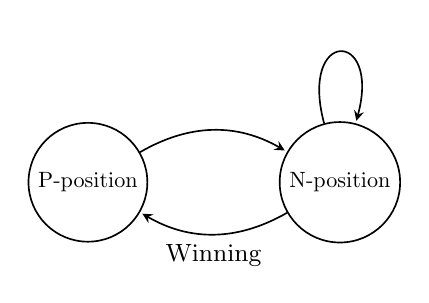
\begin{tikzpicture}
        [> = stealth,
            shorten > = 1pt,
            auto,
            node distance = 4cm,
            semithick,
            main node/.style = {circle, draw, scale=0.8}]

        \node[main node] (P) {P-position};
        \node[main node] (N) [right of=P] {N-position};

        \path[->]
        (P) edge [bend left] node {} (N)
        (N) edge [loop above] node {} (N)
        (N) edge [bend left] node [font=\small] {Winning} (P);
    \end{tikzpicture}
\end{center}

Therefore \textbf{a player starting from an N-position wins!}

If a player finds themselves in an N-position, they have the upper hand because they can force the game into a state (P-position) where their opponent is guaranteed to lose \textbf{if both play optimally}.

On the other hand, a player in a P-position is in trouble, because they are essentially doomed to lose \textbf{if the opponent plays optimally}.

\begin{definition}[Nim Game]
    The Nim game\footnote{Nim is intended to mean "Removing Game"} is defined as $(n_1, \ldots ,n_k)$ where $n_i$ is a positive integer for all $i$. At her turn any player is supposed to take one (and only one) $n_i$ and substitute it with $\hat{n} < n$.

    The winner is the player who arrives at the position $(0,0,\ldots,0)$
\end{definition}

We need to define the $\oplus $ operator on $\mathbb{N} = \{1,2, \ldots, n, \ldots\}$ for $[n_1]_2, [n_2]_2 \in \mathbb{N}$ (where $[n]_2$ is the binary representation of $n$):
\[
    [n_1]_2 \oplus [n_2]_2 = \text{sum without carry}
\]
\begin{example}
    The $\oplus$ operator applied to 1,2,4 and 1:
    \begin{align*}
        [1]_2 & = 0 \; 0 \; 1                 \\
        [2]_2 & = 0 \; 1 \; 0                 \\
        [4]_2 & = 1 \; 0 \; 0                 \\
        [1]_2 & = 0 \; 0 \; 1                 \\
        \multicolumn{2}{c}{\rule{5em}{0.4pt}} \\
        [6]_2 & = 1 \; 1 \; 0
    \end{align*}
    That is: $n_1 \oplus n_2 \oplus n_3 \oplus n_4 = 6$
\end{example}

\begin{definition}[Group]
    A nonempty set $A$ with a binary operation $\cdot$ defined on it is called a group provided that the following properties hold:
    \begin{enumerate}
        \item \textbf{Closure}: For all $a, b \in A$, $a \cdot b \in A$
        \item \textbf{Associativity}: For all $a, b, c \in A$, $(a \cdot b) \cdot c = a \cdot (b \cdot c)$
        \item \textbf{Identity Element}: There exists an (unique) element $e \in A$ such that for all $a \in A$, $a \cdot e = e \cdot a = a$
        \item \textbf{Inverse Element}: For all $a \in A$ there exists an (unique) element $a^{-1} \in A$ such that $a \cdot a^{-1} = a^{-1} \cdot a = e$
    \end{enumerate}

    If the group is commutative, i.e. $a \cdot b = b \cdot a$ for all $a, b \in A$, then it is called an \textbf{abelian group}
\end{definition}

\begin{example} Examples of abelian groups are:
    \begin{itemize}
        \item The set of integers $\mathbb{Z}$ with the operation of addition
        \item The set of real numbers $\mathbb{R}$ excluded 0 with the operation of multiplication
    \end{itemize}
\end{example}
\begin{proposition}
    Let $(A, \cdot)$ be a group. Then the \textbf{cancellation law} holds:
    \[
        \cancel{a} \cdot b = \cancel{a} \cdot c \implies b = c
    \]
\end{proposition}
\begin{proof}
    By multiplying by $a^{-1}$ both sides of the equation $a\cdot b = a\cdot c$, one obtains $a^{-1}a\cdot b = a^{-1} a\cdot c$. Then, insofar $a^{-1}$ is the \textit{inverse} of $a$, this expression reduces to $e\cdot b = e\cdot c$, which by the property of the identity $e$ is exactly equal to $b = c$.
\end{proof}

\newpage

\begin{proposition}
    The set of the natural numbers with operation $\oplus$ is an abelian group
\end{proposition}
\begin{proof}
    The identity element is of course $0$. The inverse of $n$ is $n$ itself: e.g.
    \begin{align*}
        [6]_2 & = 1 \; 1 \; 0                 \\
        [6]_2 & = 1 \; 1 \; 0                 \\
        \multicolumn{2}{c}{\rule{5em}{0.4pt}} \\
        [0]_2 & = 0 \; 0 \; 0
    \end{align*}
    Associativity and commutativity of $\oplus$ are easy to show.
\end{proof}
Therefore the cancellation law holds for the $\oplus$ operator.

\begin{theorem}[Bouton Theorem]
    In the Nim game the position $(n_1,n_2,...,n_k)$ is a \textbf{P-position} if and only if
    \begin{equation*}
        n_1 \oplus n_2 \oplus \ldots \oplus n_k = 0
    \end{equation*}
\end{theorem}
\begin{proof}
    Let's prove the theorem by demostrating that it follows the three properties of the P-positions and N-positions:
    \begin{itemize}
        \item \textbf{Terminal Position $(0,0, \ldots, 0)$ is a P-position}: zero Nim-sum
        \item \textbf{Positions with $n_1 \oplus n_2 \oplus \ldots \oplus n_N = 0$ go only to positions with non-zero Nim-sum}:\\
              Suppose that the next position $(\hat{n_1}, n_2, \ldots, n_N)$ is such that
              \begin{equation*}
                  \hat{n_1} \oplus n_2 \oplus \ldots \oplus n_N = 0 = n_1 \oplus n_2 \oplus \ldots \oplus n_N
              \end{equation*}
              By the \textbf{cancellation law} we have that $\hat{n_1} = n_1$ which is impossible because the rules of the game require $\hat{n_1} < n_1$ (we can only take away a thing)
        \item \textbf{Positions with $n_1 \oplus n_2 \oplus \ldots \oplus n_N \neq 0$ can go to position with zero Nim-sum}:\\
              We simply have to prove that exists a way to reach a position with zero Nim-sum from a non-zero Nim-sum position:\\
              Let $z = n_1 \oplus n_2 \oplus \ldots \oplus n_N \neq 0$. Take a pile having 1 inthe first column on the left of the expansion of $z$ and put $0$ there; then go right, leaving unchanged digits corresponding to $0$ and changing them otherwise. Provably, the result is smaller than the original number: Let's use $[4]_2, [6]_2, [5]_2$ and remove 1 from the first column (from left to right): $[3]_2, [6]_2, [5]_2$, as we can se we go from a non-zero Nim-sum to a zero Nim-sum
    \end{itemize}
\end{proof}

\section{Strategic Form}
in Backward induction a move must be specified at any node. Let $P_i$ be the set of all the nodes where player $i$ is called upon to make a move

\begin{definition}
    Let $P_i$ be the set of all the nodes where player $i$ is called upon to make a move
    \begin{itemize}
        \item A \textbf{pure strategy} for player $i$ is a function defined on the set $P_i$, associating to each node $v$ in $P_i$ a child $x$, or equivalently an edge $(v,x)$
        \item A \textbf{mixed strategy} is a probability distribution on the set of the pure strategies
    \end{itemize}
\end{definition}

When a player has n pure strategies, the set of her mixed strategies is
\[
    \Sigma_n := \left\{ p = ( p_1, p_2, \ldots, p_n) : p_i \geq 0, \sum_{i=1}^n p_i = 1 \right\}
\]
$\Sigma_n$ is the fundamental simplex in n-dimensional space

\begin{example}
    These is the representation of the same game both in extensive form and in strategic form

    \begin{minipage}{0.40\textwidth}
        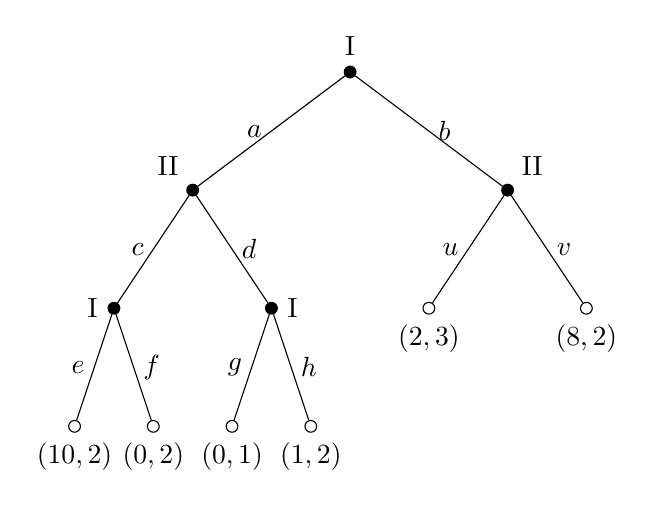
\begin{tikzpicture}
            \tikzstyle{solid node}=[circle,draw,inner sep=1.5,fill=black]
            \tikzstyle{hollow node}=[circle,draw,inner sep=1.5]
            \tikzstyle{level 1}=[level distance=15mm,sibling distance=40mm]
            \tikzstyle{level 2}=[level distance=15mm,sibling distance=20mm]
            \tikzstyle{level 3}=[level distance=15mm,sibling distance=10mm]

            \node(0)[solid node,label=above:{I}]{}
            child{node[solid node,label=above left:{II}]{}
            child{node[solid node,label=left:{I}]{}
            child{node[hollow node,label=below:{$(10,2)$}]{}
            edge from parent node[left]{$e$}}
            child{node[hollow node,label=below:{$(0,2)$}]{}
            edge from parent node[right]{$f$}}
            edge from parent node[left]{$c$}
            }
            child{node[solid node,label=right:{I}]{}
            child{node[hollow node,label=below:{$(0,1)$}]{}
            edge from parent node[left]{$g$}}
            child{node[hollow node,label=below:{$(1,2)$}]{}
            edge from parent node[right]{$h$}}
            edge from parent node[right]{$d$}
            }
            edge from parent node[left]{$a$}
            }
            child{node[solid node,label=above right:{II}]{}
            child{node[hollow node,label=below:{$(2,3)$}]{}
            edge from parent node[left]{$u$}}
            child{node[hollow node,label=below:{$(8,2)$}]{}
            edge from parent node[right]{$v$}}
            edge from parent node[right]{$b$}
            };
        \end{tikzpicture}
    \end{minipage}
    \hfill
    \begin{minipage}{0.40\textwidth}
        \begin{tabular}{|c|c|c|c|c|}
            \hline
                  & $cu$     & $cv$     & $du$    & $dv$    \\\hline
            $aeg$ & $(10,2)$ & $(10,2)$ & $(0,1)$ & $(0,1)$ \\\hline
            $aeh$ & $(10,2)$ & $(10,2)$ & $(1,2)$ & $(1,2)$ \\\hline
            $afg$ & $(0,2)$  & $(0,2)$  & $(0,1)$ & $(0,1)$ \\\hline
            $afh$ & $(0,2)$  & $(0,2)$  & $(1,2)$ & $(1,2)$ \\\hline
            $beg$ & $(2,3)$  & $(8,2)$  & $(2,3)$ & $(8,2)$ \\\hline
            $beh$ & $(2,3)$  & $(8,2)$  & $(2,3)$ & $(8,2)$ \\\hline
            $bfg$ & $(2,3)$  & $(8,2)$  & $(2,3)$ & $(8,2)$ \\\hline
            $bfh$ & $(2,3)$  & $(8,2)$  & $(2,3)$ & $(8,2)$ \\
            \hline
        \end{tabular}
    \end{minipage}

    All combinations are listed even if equivalent (e.g. strategies $beg, beh, \ldots$ for Player 2).

    The table has repeated pairs: different strategies can lead to the same outcomes
    \begin{itemize}
        \item Extensive form: the different moves of the players are presented in sequence
        \item Strategic form: all strategies of the players are presented at the same time
    \end{itemize}
\end{example}

One can reformulate von Neumann’s theorem in terms of strategies as follows:

\begin{theorem}[Von Neumann (Strategic Form)]
    In the chess game one of the following alternatives holds:
    \begin{itemize}
        \item White has a winning strategy
        \item Black has a winning strategy
        \item both players have a strategy leading them at least to a tie
    \end{itemize}
\end{theorem}

Graphically The 3 outcomes can be represented as follows:
\vspace{0.5cm}
\begin{center}
    \begin{minipage}{0.3\textwidth}
        \centering
        \begin{tabular}{|c|c|c|c|c|}
            \hline
                     & $1$      & $2$      & $\ldots$ & $K$      \\\hline
            $a$      & $\ldots$ & $\ldots$ & $\ldots$ & $\ldots$ \\\hline
            $b$      & $\ldots$ & $\ldots$ & $\ldots$ & $\ldots$ \\\hline
            $c$      & $W $     & $W$      & $\ldots$ & $W$      \\\hline
            $\ldots$ & $\ldots$ & $\ldots$ & $\ldots$ & $\ldots$ \\\hline
            $K$      & $\ldots$ & $\ldots$ & $\ldots$ & $\ldots$ \\
            \hline
        \end{tabular}
        \vspace{0.5cm}
        \par{White has a winning strat (i.e a raw with all $W$)}
    \end{minipage}
    \hfill
    \begin{minipage}{0.3\textwidth}
        \centering
        \begin{tabular}{|c|c|c|c|c|}
            \hline
                     & $1$      & $2$      & $\ldots$ & $K$      \\\hline
            $a$      & $\ldots$ & $B$      & $\ldots$ & $\ldots$ \\\hline
            $b$      & $\ldots$ & $B$      & $\ldots$ & $\ldots$ \\\hline
            $c$      & $\ldots$ & $B$      & $\ldots$ & $\ldots$ \\\hline
            $\ldots$ & $\ldots$ & $\ldots$ & $\ldots$ & $\ldots$ \\\hline
            $K$      & $\ldots$ & $B$      & $\ldots$ & $\ldots$ \\
            \hline
        \end{tabular}
        \vspace{0.5cm}
        \par{Black has a winning strat (i.e a col with all $B$)}
    \end{minipage}
    \hfill
    \begin{minipage}{0.3\textwidth}
        \centering
        \begin{tabular}{|c|c|c|c|c|}
            \hline
                     & $1$      & $2$      & $\ldots$ & $K$      \\\hline
            $a$      & $\ldots$ & $B$      & $\ldots$ & $\ldots$ \\\hline
            $b$      & $\ldots$ & $T$      & $\ldots$ & $\ldots$ \\\hline
            $c$      & $W$      & $T$      & $\ldots$ & $W$      \\\hline
            $\ldots$ & $\ldots$ & $\ldots$ & $\ldots$ & $\ldots$ \\\hline
            $K$      & $\ldots$ & $T$      & $\ldots$ & $\ldots$ \\
            \hline
        \end{tabular}
        \vspace{0.5cm}
        \par{The outcome is (at least) a tie for both players}
    \end{minipage}
\end{center}
\vspace{0.5cm}
So, for von Neumann's theorem outcomes like this are not possibile:
\vspace{0.5cm}
\begin{center}
    \begin{tabular}{|c|c|c|c|c|}
        \hline
                 & $1$      & $2$      & $\ldots$ & $K$      \\\hline
        $a$      & $\ldots$ & $B$      & $\ldots$ & $\ldots$ \\\hline
        $b$      & $\ldots$ & $T$      & $\ldots$ & $\ldots$ \\\hline
        $c$      & $T$      & $W$      & $\ldots$ & $B$      \\\hline
        $\ldots$ & $\ldots$ & $\ldots$ & $\ldots$ & $\ldots$ \\\hline
        $K$      & $\ldots$ & $T$      & $\ldots$ & $\ldots$ \\
        \hline
    \end{tabular}
\end{center}
\vspace{0.5cm}
We can't have a strategy \textit{(a row, or a column)} with all 3 possibile outcomes ($W$, $B$, $T$)

\begin{remark}
    If $P_i = \{v_1, \ldots , v_k \}$ and $v_j$ has $n_j$ children, then the number of strategies of Player $i$ is $n_1\cdot n_2\cdot \ldots\cdot n_k$
\end{remark}

This shows that the number of strategies even in short games is usually very high. For instance, if Tic-Tac-Toe is stopped after three moves, the first player has (without exploiting symmetries) $9\cdot 7^{(8\cdot 9)}$ strategies

\section{Games with imperfect information}
Sometimes players must make moves at the same time, and so they cannot have full knowledge of each other’s moves. This can be still represented with a tree.

\textit{Dashed line: the player does not know exactly which vertex she finds herself in}
\begin{center}
    \begin{tikzpicture}
        \tikzstyle{solid node}=[circle,draw,inner sep=1.5,fill=black]
        \tikzstyle{level 1}=[level distance=20mm,sibling distance=60mm]
        \tikzstyle{level 2}=[level distance=20mm,sibling distance=30mm]
        \tikzstyle{level 3}=[level distance=20mm,sibling distance=15mm]

        % Root node and main tree structure
        \node(0)[solid node]{}
        child{node[solid node](n1l){}
                child{node[solid node](n2ll){}
                        child{node[solid node]{}}
                        child{node[solid node]{}}
                        edge from parent
                    }
                child{node[solid node](n2lr){}
                        child{node[solid node]{}}
                        child{node[solid node]{}}
                        edge from parent
                    }
                edge from parent
            }
        child{node[solid node](n1r){}
                child{node[solid node](n2rl){}
                        child{node[solid node]{}}
                        child{node[solid node]{}}
                        edge from parent
                    }
                child{node[solid node](n2rr){}
                        child{node[solid node]{}}
                        child{node[solid node]{}}
                        edge from parent
                    }
                edge from parent
            };

        % Information sets (dashed lines)
        \draw[dashed] (n1l) -- (n1r);
        \draw[dashed] (n2ll) -- (n2lr);
        \draw[dashed] (n2rl) -- (n2rr);
    \end{tikzpicture}
\end{center}
\begin{definition}[Information Set]
    An information set for a player $i$ is a pair $(U_i , A(U_i))$ with the following properties:
    \begin{enumerate}
        \item $U_i \subset P_i$ is a nonempty set of vertices $v_1,\ldots,v_k$
        \item each $v_j \in U_i$ has the same number of children
        \item $A_i(U_i)$ (Available Moves) is a partition of the children of $v_1 \cup \ldots \cup v_k$ with the property that each element of the partition contains exactly one child of each vertex $v_j$
    \end{enumerate}
    Accordingly, player $i$ knows to be in $U_i$, but not in which vertex she is.
    The partition yields the choice function, meaning that each set in $A_i(U_i)$ represents an available move for the player
\end{definition}

\begin{definition}[Extensive Game with Imperfect Information]
    An extensive Game with Imperfect Information is constituted by
    \begin{itemize}
        \item A finite set $N = \{1, \ldots, n\}$ of players
        \item A game tree $(V, E, x_0)$
        \item A partition of the vertices that are not leaves into sets $P_1, P_2, \ldots, P_{n+1}$ of the vertices that are not leaves
        \item A partition $(U_i^j), j=1,\ldots,k_i$ of the set $P_i$ for all $i$ with $(U_i^j, A_i^j)$ information set for all players $i$ for all vertices $j$ (with the same number of children)
        \item A probability distribution, for each vertex in $P_{n+1}$, defined on the edges going from the vertex to its children
        \item An n-dimensional vector attached to each leaf (i.e. the points associated to each player)
    \end{itemize}
\end{definition}

\newpage

\begin{definition}
    A \textbf{pure strategy for player $i$ in an imperfect information game} is a function defined on the collection $\mathcal{U}$ his information sets and assigning to each $U_i$ in $\mathcal{U}$ element of the partition $A(U_i)$.

    A mixed strategy is a probability distribution over the pure strategies.
\end{definition}
\begin{remark}
    A game of perfect information is a particular game of imperfect information where all information sets of all players are singletons (i.e. consist of only one vertex)
    \begin{equation*}
        \text{Perfect Information} \subset \text{Imperfect Information}
    \end{equation*}
\end{remark}
\end{document}